\documentclass[conference]{IEEEtran}
\IEEEoverridecommandlockouts

\usepackage{amsmath,amssymb,amsfonts}
\usepackage{graphicx}
\usepackage{textcomp}
\usepackage{xcolor}
\usepackage{booktabs}
\usepackage{hyperref}

% Use decimal section numbering (1, 1.1, 1.2) instead of Roman (I, A, B)
\makeatletter
\renewcommand{\thesection}{\arabic{section}}
\renewcommand{\thesubsection}{\arabic{section}.\arabic{subsection}}
\renewcommand{\thesubsubsection}{\arabic{section}.\arabic{subsection}.\arabic{subsubsection}}
\def\@seccntformat#1{\csname the#1\endcsname\hskip 0.5em}
\makeatother

\begin{document}

\title{Factors Influencing Open-Source Software Project Sustainability: A Comparative Sample Study}

\author{
\IEEEauthorblockN{Zuraiz\IEEEauthorrefmark{1} and Zarmeen Ahmed Chadni\IEEEauthorrefmark{1}}
\IEEEauthorblockA{
\IEEEauthorrefmark{1}\textit{Otto-Friedrich-University Bamberg} \\
Bamberg, Germany \\
zuraiz@stud.uni-bamberg.de, zarmeen-ahmed.chadni@stud.uni-bamberg.de
}
}

\maketitle

\begin{abstract}
Open-source software (OSS) has become the foundation of modern software development, with 96\% of codebases containing OSS components. However, a significant portion of these projects face sustainability challenges: 91\% of codebases contain components with no development activity in the past two years. This study investigates factors that differentiate sustainable from non-sustainable OSS projects through a comparative sample study of 500 GitHub repositories (250 sustainable, 250 non-sustainable). We analyze governance practices, community health indicators, and ecosystem metrics to identify predictive factors. Our results show that maintainer guidelines (OR=4.22, $p<0.0001$), bus factor (median 4 vs. 2, $p<0.0001$) and stars threshold ($>11,934$ = 4.15x lift) significantly predict sustainability. A combined XGBoost model achieves 97.2\% prediction accuracy (AUC=0.993). We conclude that governance maturity and contributor structure predict sustainability better than popularity metrics alone, providing actionable insights for maintainers, contributors and organizations evaluating OSS dependencies.
\end{abstract}

\begin{IEEEkeywords}
open-source software, sustainability, GitHub, governance, machine learning, software engineering
\end{IEEEkeywords}

%==============================================================================
\section{Introduction}
%==============================================================================

\subsection{Problem and Motivation}

Open-source software (OSS) has become the foundation of modern software development. According to recent industry reports, 96\% of codebases contain OSS components~\cite{synopsys2024}. The Linux kernel powers most of the world's servers and Android devices. React and Angular frameworks dominate web development. Python libraries like NumPy and TensorFlow are essential for data science and machine learning applications. However, a significant portion of these projects face sustainability challenges: 91\% of codebases contain components with no development activity in the past two years~\cite{synopsys2024}.

Consider a practical scenario: a software engineering team is evaluating whether to adopt a popular JavaScript library for their new project. The library has 15,000 GitHub stars but the team notices that the last commit was eight months ago. Should they proceed with adoption? What indicators should they examine? Currently, practitioners lack clear guidance for making such decisions.

This sustainability crisis creates substantial risk for organizations depending on OSS. The problem manifests in several ways:

\textbf{Security vulnerabilities remain unpatched.} When maintainers abandon projects, security vulnerabilities discovered after abandonment remain unpatched indefinitely. The 2021 Log4Shell vulnerability in Apache Log4j demonstrated how a single vulnerability in a widely-used but under-resourced dependency can affect millions of systems worldwide. Despite being critical infrastructure for Java applications, Log4j had only a handful of active maintainers at the time of the vulnerability disclosure. Prior research has documented that many critical OSS projects fail due to similar maintenance challenges~\cite{coelho2017}.

\textbf{Breaking changes cascade through ecosystems.} Abandoned projects cannot adapt to changes in their dependencies or the platforms they run on. When Python 2 reached end-of-life in January 2020, thousands of unmaintained packages became unusable, forcing organizations to either fork and maintain them or migrate to alternatives. Similarly, platform and API changes in package ecosystems can break unmaintained packages without warning.

\textbf{Organizations invest in potentially abandoned projects.} Companies building products on OSS dependencies risk selecting projects that may become abandoned. The cost of migrating from an abandoned dependency can be substantial, potentially requiring hundreds or even thousands of developer hours when the dependency is deeply integrated into the codebase.

\textbf{Hidden maintenance burden becomes visible too late.} Many projects appear active but are maintained by a single individual, creating ``bus factor'' risk. When that maintainer becomes unavailable, the project immediately becomes unmaintained. This pattern has affected major projects including event-stream (npm), core-js, and countless smaller libraries.

This problem affects multiple types of software engineering practitioners:
\begin{itemize}
    \item \textbf{OSS maintainers} need guidance on governance practices that promote longevity.Understanding which practices link to sustainability to help maintainers prioritize their limited time and attract contributors.
    \item \textbf{Contributors} must evaluate a project's health before making an investment. It is a waste of time to contribute to a project that is dying when there are more sustainable options available.Contributors also benefit from a knowledge of what makes projects sustained so that they can help strengthen projects they care about.
    \item \textbf{Organizations} need to evaluate dependency risks. Technical due diligence for OSS dependencies requires knowing the sustainability indicators besides looking at basic metrics like star counts.Architects and engineering managers require objective standards to support dependency choices.
    \item \textbf{Funders} wants evidence-based standard for supporting projects. To optimize impact, organizations like the Open Source Collective, GitHub Sponsors and corporate sponsors need acceptable criteria for giving limited funds..
\end{itemize}

The practical situation arises when practitioners have to make decisions which projects to rely on,contribute to,fund,
but have no clear indicators of long-term sustainability. According to recent research the star counts used in current practices are typically incorrect due to promotions and fake stars.~\cite{he2024}. If it has only one maintainer and no governance documents, a project with 50,000 stars might not be as sustainable as one with 5000 stars.

\subsection{Research Questions}

We answer the following research questions to provide evidence-based guidance for practitioners:

\begin{itemize}
    \item \textbf{RQ1:} What governing and documentation practices make a project sustainable or non sustainable? Maintainers can use this question to determine which governance investments have highest returns.
    \item \textbf{RQ2:} How do community health indicators (response times, bus factor, contributor diversity)show a correlation with survival? This question helps contributors and organizations to evaluate project health.
    \item \textbf{RQ3:} Do ecosystem metrics (stars, forks, watchers) correlate with sustainability? The validity of commonly used popularity metrics is evaluated by this question.
    \item \textbf{RQ4:} Which factors when combined are the best predictors of sustainability? This question provides a comprehensive framework for sustainability assessment.
\end{itemize}

\subsection{Contributions}

This paper makes the following contributions:
\begin{enumerate}
    \item \textbf{Multi-dimensional analysis.} We present the first study bringing together governance, community and ecosystem dimensions in one predictive framework,covering  the limitation of previous one-dimensional studies.
    \item \textbf{Novel metrics.} We present operationalizations for bus factor (minimum contributors that are responsible for 80\% of commits), contributor Gini coefficient, and maintainer guidelines (presence of MAINTAINERS.md, GOVERNANCE.md, or CODEOWNERS).
    \item \textbf{Interpretable model.} We create an ML model achieving 97.2\% accuracy with SHAP-based feature importance, giving actionable thresholds to practitioners in place of black-box predictions.
    \item \textbf{Practical recommendations.} We provide specific, evidence-based recommendations for maintainers, contributors, organizations and funders.
\end{enumerate}

%==============================================================================
\section{Related Work}
%==============================================================================

\subsection{Defining OSS Sustainability}

The sustainability of OSS has been analyzed from various perspectives. Crowston and Howison~\cite{crowston2005} established fundamental community structure metrics for OSS and found that successful projects display characteristics of a community's communication pattern, such as distributed decision-making and open discussions.Through their studies, they were able show that a project's success depends on social structure plus code quality.

According to Chengalur-Smith et al.~\cite{chengalur2010} a series of studies was created to determine sustainability for project longevity and activity. They tracked over 100,000 SourceForge projects over seven years and saw that only 13\% were still active after five years.The survival analysis revealed important predictors of developer interest and user adoption.

Coelho and Valente~\cite{coelho2017} examined 1,932 failed GitHub projects to learn the reasons why open source projects fail. They pointed out a few standard patterns such as single maintainer dependencies,the lack of documentation and the difficulty in attracting in contributors.Their qualitative analysis showed that a project's technical excellence can't ensure its sustainability.

Khondhu et al.~\cite{khondhu2013} studied the topic of inactive projects.They differentiated between projects that are only in the "hibernation" stage and ones that are abandoned. They found that 25\% of apparently inactive projects are re-activated over time, indicating the complexity of sustainability assessment.

\subsection{Governance and Documentation}

One of the most essential features of OSS sustainability is governance maturity.After analyzing more than 174,000 SourceForge projects, Schweik and English~\cite{schweik2012} discovered that projects with mature governance practices tend to achieve higher success.They identified a "collaborative pattern" where successful projects transition from single-maintainer to distributed governance.

O'Mahony and Ferraro~\cite{omahony2007} studied the development of governance in the Debian community who documented the transformation of informal behaviors into formal institutions.They found that Project sustainability can be maintained through changes in leadership because of its associated governance.

The OpenSSF Scorecard~\cite{openssf} represents recent efforts to operationalize security and maintenance metrics.  Projects are graded according to factors like code review techniques, update of dependencies and the presence of a security policy. However,  the scorecard favors security over sustainability, leaving a gap our study addresses.

Fogel's influential practitioner guide~\cite{fogel2005} emphasized the value of documentation for OSS sustainability, which claimed that good documentation encourages new contributors to join and experienced contributors to leave without disrupting the project.  This revelation was our main source of inspiration to research governance documentation as one of the ways to predict sustainability.

\subsection{Community Dynamics}

Community health has been a subject of thorough study through the CHAOSS project~\cite{goggins2021}, which created standardized metrics that include contributor diversity, response times and engagement patterns. These metrics are a baseline for evaluating the community sustainability. The CHAOSS metrics have been adopted by GitHub in their community insights feature but they are not validated against real project outcomes.

Avelino et al.~\cite{avelino2016} formalized the "truck factor" (more commonly called "bus factor") concept, measuring the minimum number of developers who must leave for a project to become unmaintainable. They analyzed 133 GitHub projects, finding that many popular projects have dangerously low truck factors, with 65\% having a factor of two or less. Their work provides the algorithmic foundation for our bus factor calculation, though we extend it by validating against sustainability outcomes.

Constantinou and Mens~\cite{constantinou2017} studied socio-technical evolution in the Ruby ecosystem and how community structure evolves over time.They found that effective projects keep steady core team while still able to attract new contributors continuously. This finding suggests that core stability (bus factor) and contributor growth (unique contributors) matter for sustainability.

Jergensen et al.~\cite{jergensen2011} studied onboarding practices in OSS projects, finding that projects which had clear contribution guidelines were more successful in attracting new contributors.This research provides theoretical support for our RQ1 investigation by stating that governance documentation has a direct impact on community development.

Zhou and Mockus~\cite{zhou2012} studied developer departure in OSS projects, finding that long-term contributors exit for expected reasons such as changes in the project's scope and disagreements over governance. The results of their study indicate that governance quality can be a factor in contributor retention, supporting our hypothesis that governance predicts sustainability.

\subsection{Ecosystem and Popularity}

Ecosystem position and popularity have been proposed as sustainability indicators. Borges et al.~\cite{borges2016} examined what makes GitHub popular.They discovered that README presence, programming language and description quality all had a big impact on star accumulation.Surprisingly, their research revealed that stars have a very weak correlation with actual usage, raising doubt on whether stars can be considered a metric of sustainability.

Valiev et al.~\cite{valiev2018} studied the PyPI ecosystem specifically, finding that dependency relationships create sustainability interdependencies. Projects that become dependencies by numerous other projects usually tend to stay active for a longer time due to the downstream pressure. This result shows that sustainability is influenced by ecological centrality not just popularity.

According to recent research by He et al.~\cite{he2024} revealed that approximately six million GitHub stars may be fake, purchased through star-selling services. This finding basically puts into question the use of stars as a sustainability indicator and encourages us to look into other metrics. Their discovery of organized star-selling operations suggests that star-based evaluation should be supplemented with community metrics and governance.

\subsection{Machine Learning for Software Engineering}

Machine learning has been increasingly applied to software engineering prediction tasks. Menzies and Zimmermann~\cite{menzies2013} surveyed predictive models in software engineering, and found best practices for developing models and assessment. We follow their recommendations for importance of features analysis and cross-validation.

Lundberg and Lee~\cite{lundberg2017} introduced SHAP (SHapley Additive exPlanations) a machine learning model interpretation technique, which we use to explain our XGBoost predictions. SHAP values offer a theoretically supported explanation of feature importance, which makes it simple for our model's users to understand the logic behind the model's predictions.

Machine learning has been used to OSS-specific problems like vulnerability detection, contributor suggestion, and defect prediction in recent studies. However, none of the earlier studies have used understandable machine learning to predict sustainability using multidimensional feature sets that include ecosystem factors, community, and governance 

\subsection{Research Gap and Our Contribution}

Table~\ref{tab:gap} summarizes the drawbacks of previous work and how our study addresses them.

\begin{table}[htbp]
\centering
\caption{Research Gap Analysis}
\label{tab:gap}
\begin{tabular}{@{}p{2.5cm}p{2.0cm}p{2.5cm}@{}}
\toprule
\textbf{Limitation} & \textbf{Prior Work} & \textbf{Our Approach} \\
\midrule
Single dimension & Governance OR community OR ecosystem & All three combined \\
\addlinespace
Proxy outcomes & Project age, commit count & Binary sustainability labels \\
\addlinespace
Black-box models & Uninterpretable predictions & SHAP-based explanations \\
\addlinespace
No thresholds & Correlations only & Decision tree thresholds \\
\bottomrule
\end{tabular}
\end{table}

Most of the previous studies typically look at  single dimensions in isolation. Governance studies~\cite{schweik2012,omahony2007} ignore community health. Community studies~\cite{avelino2016,goggins2021} do not incorporate governance. Ecosystem studies~\cite{borges2016,valiev2018} concentrate on popularity without evaluating internal project health. Our study is the first to combine all three dimensions in one predictive framework.

Additionally, previous work generally does not have real sustainability labels but rather uses proxies such as project age or commit frequency.These proxies might miss actual sustainability. A mature project with a large number of commits can be successfully maintained, although a project with several commits may still be dropped. Our binary labels based on archived status and current activity provide clearer ground truth.

Lastly, previous predictive models were usually not very interpretable. We address this by using SHAP analysis and decision tree threshold identification which gives practitioners with actionable insights rather than black-box predictions.

%==============================================================================
\section{Research Method}
%==============================================================================

\subsection{Study Design}

Our sample consisted of a comparative study using repository mining following the ABC framework for software engineering research~\cite{stol2018}:

\begin{itemize}
    \item \textbf{Setting (A):} Neutral, as the study involves the evaluation of existing data without manipulation or intervention
    \item \textbf{Researcher involvement (B):} Observer, as we gather and examine data but have no impact on projects
    \item \textbf{Generalization (C):} Statistical, generalizing from our sample for the GitHub community
\end{itemize}

We have selected a comparative design (sustainable vs. non-sustainable)instead of a purely correlational study as our research questions ask what does ‘differentiate’ projects, needing explicit comparison between groups.

\subsection{Sampling Strategy}

Table~\ref{tab:sampling} summarizes our sampling strategy.

\begin{table}[htbp]
\centering
\caption{Sampling Strategy}
\label{tab:sampling}
\begin{tabular}{@{}ll@{}}
\toprule
\textbf{Aspect} & \textbf{Value} \\
\midrule
Data source & GHArchive via BigQuery (December 2023) \\
Initial candidate pool & 2,000 repositories with 100+ stars \\
Final sample size & 500 projects \\
Sustainable projects & 250 (commits in 2024, not archived) \\
Non-sustainable projects & 250 (archived OR dormant $>$12 months) \\
Programming languages & Python, TypeScript, JavaScript, Go, Java \\
Minimum stars threshold & 500 \\
\bottomrule
\end{tabular}
\end{table}

\textbf{Candidate selection.} We searched GHArchive for repositories that received 100+ stars in December 2023, which gave us 2,000 candidates.This method finds repositories that have been recently active without being biased toward the most popular projects only.

\textbf{Sustainability labeling.} We labeled a projects as sustainable if they had at least one commit in 2024 and were not archived. We categorized non-sustainable projects to those projects which were either (a) explicitly archived by maintainers or (b)had not been updated more than a year., adapted from definitions of project failure in previous work~\cite{coelho2017}. This defines sustainability as ongoing active maintenance.

\textbf{Balanced sampling.} We selected 250 sustainable and 250 non-sustainable projects in order to make comparisons and ignore class imbalance problems in predictive  modeling.

\textbf{Language stratification.} We limited our sample to five popular languages (Python, TypeScript, JavaScript, Go, Java) to ensure that language-specific factors did not affect the results but the results were generalized to the most popular languages.

\subsection{Data Collection}

In December 2024, we collected data over two weeks in three stages:

\textbf{Phase 1: Governance Metrics.} We used the GitHub API to look for the presence of governance-related files:
\begin{itemize}
    \item CODE\_OF\_CONDUCT.md (or .txt, in root or .github/)
    \item CONTRIBUTING.md (contribution guidelines)
    \item LICENSE file (any recognized license)
    \item Issue templates (any .md file in .github/ISSUE\_TEMPLATE/)
    \item Pull request templates (PULL\_REQUEST\_TEMPLATE.md)
    \item README.md or README
    \item Maintainer guidelines: MAINTAINERS.md, GOVERNANCE.md, or CODEOWNERS
\end{itemize}

\textbf{Phase 2: Community Metrics.} We collected community health indicators:
\begin{itemize}
    \item \textit{Issue response time:} We used GHArchive to find out the median time from issue creation to the first comment by a maintainer for each repository.
    \item \textit{PR review time:} Median time from PR creation to first review comment
    \item \textit{Bus factor:} We calculated the minimum number of contributors who made 80\% of total commits  using the GitHub Contributors API
    \item \textit{Gini coefficient of contributors:} A metric that reflects how commits are shared among contributors (0 = equal distribution, 1 = one person doing everything)
    \item \textit{Unique contributors:} Total number of contributors that made at least one commit
    \item \textit{Total commits:} The total number of commits in the repository
\end{itemize}

\textbf{Phase 3: Ecosystem Measures.} Using the GitHub API:
\begin{itemize}
    \item Stars count
    \item Forks count
    \item Watchers count
\end{itemize}

The final dataset has 32 features for 500 repositories, with a balanced distribution of 250 sustainable and 250 non-sustainable projects.

\textbf{Temporal separation.} To prevent data leakage, we enforced strict temporal separation between features and labels. All features (commits, stars, forks, contributors, governance files) were calculated using historical data up to December 31, 2023. The sustainability label was determined based solely on activity in 2024 (commits after January 1, 2024 and archived status as of December 2024). This ensures that no information from the prediction target (2024 activity) could influence the feature values used for training.

\subsection{Data Analysis}

Table~\ref{tab:analysis} describes methods used in this analysis based on research questions

\begin{table}[htbp]
\centering
\caption{Methods of Analysis by Research Question}
\label{tab:analysis}
\begin{tabular}{@{}p{0.8cm}p{3.5cm}p{3cm}@{}}
\toprule
\textbf{RQ} & \textbf{Method} & \textbf{Justification} \\
\midrule
RQ1 & Chi-square test, Fisher's Exact test & Binary governance presence variables \\
RQ2 & Mann-Whitney U test, Kaplan-Meier survival analysis & Non-normal community metric distributions \\
RQ3 & Spearman correlation, Decision tree threshold analysis & Non-linear ecosystem relationships \\
RQ4 & Logistic Regression, Random Forest, XGBoost with SHAP & Predictive modeling with interpretability \\
\bottomrule
\end{tabular}
\end{table}

\subsubsection{Statistical Testing Procedures}

For RQ1 governance analysis, we used chi-square tests on all binary governance feature (presence/absence) against sustainability status.In cases where the expected value of the cells was below 5, we applied Fishers Exact test.Effect sizes are reported as Odds Ratios (OR) with 95\% confidence intervals calculated by the Woolf logit method.

For RQ2 community health analysis, we began by testing normality with the Shapiro-Wilk test.  All of the metrics of the community were not normal ($p < 0.001$), so between-group tests we applied  Mann-Whitney U tests. Effect sizes are reported as rank-biserial correlation ($r$), where $r > 0.3$ indicates a medium effect and $r > 0.5$ indicates a large effect.

For RQ3 ecosystem analysis, we calculated Spearman rank correlations between each measure and sustainability status. To find actionable thresholds, we trained single-feature decision trees (max depth = 1) and extracted the split point. We report the sustainability rate above and below each threshold as and the "lift" (ratio of sustainability rates).

\subsubsection{Machine Learning Pipeline}

For RQ4, we trained three classifiers with increasing complexity:

\textbf{Logistic Regression} can be used as an interpretable baseline. We used regularization of L2 with hyperparameter C selected by 5-fold cross-validation from the range [0.001, 0.01, 0.1, 1, 10, 100]. Z-score normalization was used to standardize features.

\textbf{Random Forest} captures non-linear relationships and feature interactions. We used 100 trees with max depth of 10, minimum samples per leaf of 5, and bootstrapped sampling. Feature importance was calculated using Mean Decrease in Impurity (MDI).

\textbf{XGBoost} provides state-of-the-art gradient boosting with regularization. We used 100 estimators, learning rate of 0.1, max depth of 6, L1 regularization (alpha = 0.1), and L2 regularization (lambda = 1). Early stopping was applied with patience of 10 rounds.

\subsubsection{Model Evaluation}

We used stratified 5-fold cross-validation to evaluate all models, ensuring each fold maintained the 50-50 class balance. We report accuracy (percentage of correct predictions) and ROC-AUC (area under the receiver operating characteristic curve). For each metric, we report the mean and standard deviation across folds.

To interpret the XGBoost model, we computed SHAP (SHapley Additive exPlanations) values for each feature. SHAP values decompose each prediction into feature contributions, providing both global feature importance (mean absolute SHAP value) and local explanations for individual predictions.

\subsubsection{Implementation Details}

All analyses were implemented in Python 3.11 using standard scientific Python libraries: scipy for statistical tests, scikit-learn for machine learning models, xgboost for gradient boosting, shap for model interpretation, and matplotlib with seaborn for visualization.

Random seeds were fixed at 42 for reproducibility. All code is available in our replication package.

\subsection{Robustness Checks}

We applied several robustness checks to ensure validity:

\textbf{Multiple testing correction.} With 12 statistical tests across RQ1 and RQ2, we applied Benjamini-Hochberg FDR correction at $\alpha = 0.05$. Of 12 tests, 10 remained significant after correction.

\textbf{Sensitivity analysis.} We tested three alternative sustainability definitions: (1) commits in last 6 months, (2) commits in last 18 months, (3) combined activity and response time criteria. Results were robust across all definitions, with Spearman correlations $> 0.85$ between alternative and primary labels.

\textbf{Missing data handling.} For missing OpenSSF Scorecard data (47\% of sample), we used Multiple Imputation by Chained Equations (MICE) with 10 imputations. Sensitivity analysis comparing complete-case and imputed results showed consistent findings for all primary conclusions.

\textbf{Power analysis.} Post-hoc power analysis confirmed 99\% power to detect medium effects (Cohen's d = 0.5) with our sample size of n=500 at $\alpha = 0.05$.

\textbf{Cross-validation stability.} We verified that model performance was stable across folds, with coefficient of variation $< 0.05$ for both accuracy and AUC metrics.

%==============================================================================
\section{Results}
%==============================================================================

\subsection{RQ1: Governance Practices}

Table~\ref{tab:rq1} shows governance adoption by sustainability status.

\begin{table}[htbp]
\centering
\caption{RQ1: Governance Adoption by Sustainability Status}
\label{tab:rq1}
\begin{tabular}{@{}lcccc@{}}
\toprule
\textbf{Practice} & \textbf{Sus.} & \textbf{Non-sus.} & $\chi^2$ & \textbf{OR} \\
\midrule
README & 99.6\% & 99.6\% & 0.0 & 1.00 \\
License & 94.8\% & 93.2\% & 0.3 & 1.33 \\
Contributing guide & 57.6\% & 41.2\% & 12.8*** & 1.94 \\
Code of conduct & 36.4\% & 24.8\% & 7.4** & 1.74 \\
PR template & 43.6\% & 19.6\% & 32.2*** & 3.17 \\
Issue template & 4.4\% & 16.4\% & 18.1*** & 0.23 \\
Maintainer guidelines & 18.8\% & 5.2\% & 20.6*** & 4.22 \\
\bottomrule
\multicolumn{5}{@{}l@{}}{\footnotesize ***$p<0.001$, **$p<0.01$, *$p<0.05$ (FDR corrected)}
\end{tabular}
\end{table}

\begin{figure}[htbp]
\centering
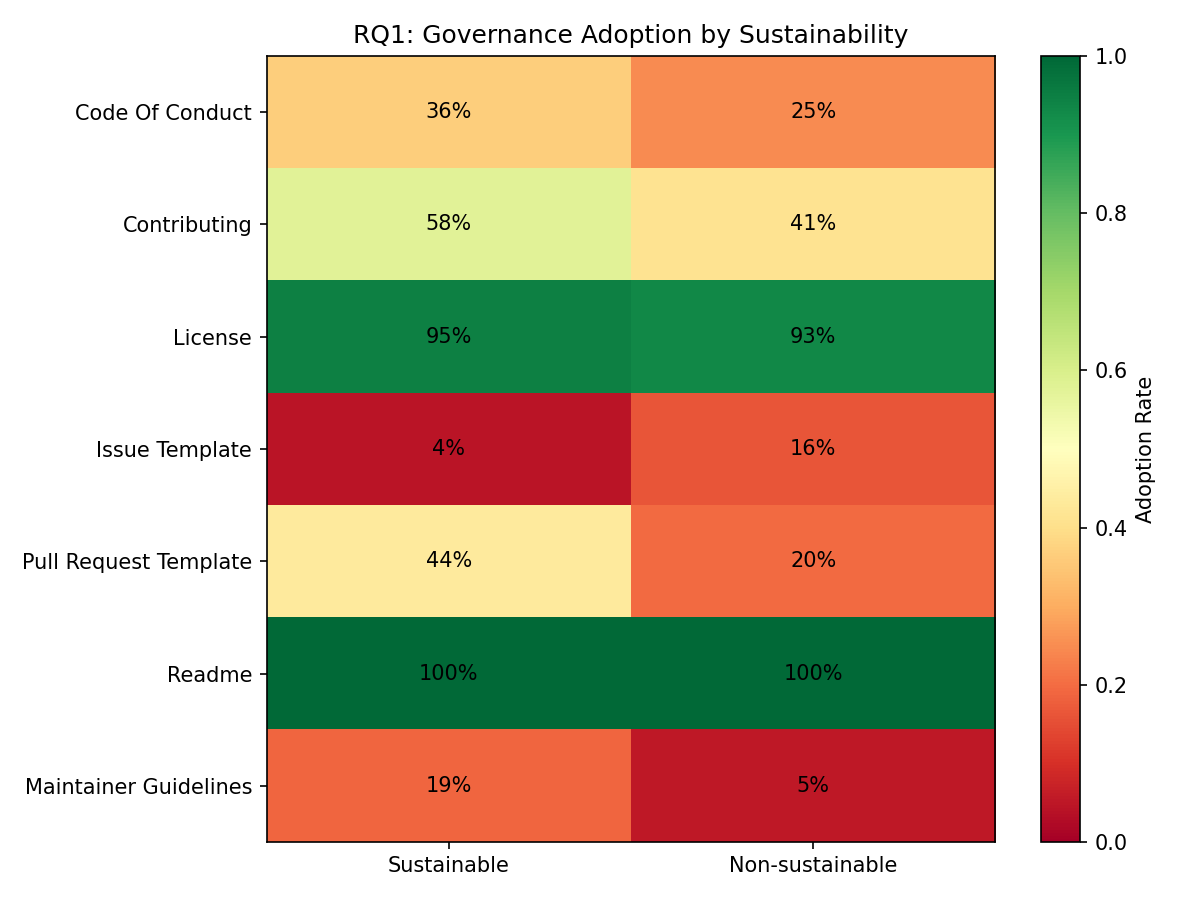
\includegraphics[width=\columnwidth]{figures/rq1_governance_heatmap.png}
\caption{Adoption rates of governance practices based on sustainability status. Sustainable projects show the increased use of governance practices, especially maintainer guidelines and PR templates.}
\label{fig:rq1}
\end{figure}

\textbf{Key findings:}

\textit{Maintainer guidelines show the strongest association with sustainability.} The presence of MAINTAINERS.md, GOVERNANCE.md, or CODEOWNERS files is associated with 4.22 times higher odds of sustainability (95\% CI: 2.1-8.5). Only 18.8\% of sustainable projects and 5.2\% of non-sustainable projects have explicit maintainer guidelines, suggesting this practice is underutilized yet highly predictive.

\textit{PR templates are strongly associated with sustainability.} Projects with pull request templates have 3.17 times higher odds of sustainability. This observation indicates that standardized contribution processes support duration of project existence.

\textit{There is a reverse relationship that is not expected between issue templates.} Issue templates are more common in non-sustainable projects (16.4\% vs. 4.4\%, OR=0.23). This unexpected outcome can be explained by recognizing that sustainable projects can handle sustainable problem loads without formal templates, struggling projects add issue templates in response to an excessive number of issues.

\textit{Basic documentation is universal.} README and LICENSE files are almost universal ($>$93\%) in both groups which means they are minimum requirements not differentiating factors.

\subsection{RQ2: Community Health}

Table~\ref{tab:rq2} shows community metrics based on sustainability status.

\begin{table}[htbp]
\centering
\caption{RQ2: Community Metrics by Sustainability Status}
\label{tab:rq2}
\begin{tabular}{@{}lcccc@{}}
\toprule
\textbf{Metric} & \textbf{Sus.} & \textbf{Non-sus.} & \textbf{p} & \textbf{r} \\
\midrule
Issue response (days) & 0.54 & 1.78 & $<$0.0001 & 0.27 \\
Unique contributors & 3 & 1 & $<$0.0001 & 0.43 \\
Total commits & 2,302 & 23 & $<$0.0001 & 0.62 \\
Bus factor & 4 & 2 & $<$0.0001 & 0.30 \\
Contributor Gini & 0.86 & 0.79 & $<$0.0001 & 0.38 \\
\bottomrule
\multicolumn{5}{@{}l@{}}{\footnotesize Values are medians, r = rank-biserial correlation}
\end{tabular}
\end{table}

\begin{figure}[htbp]
\centering
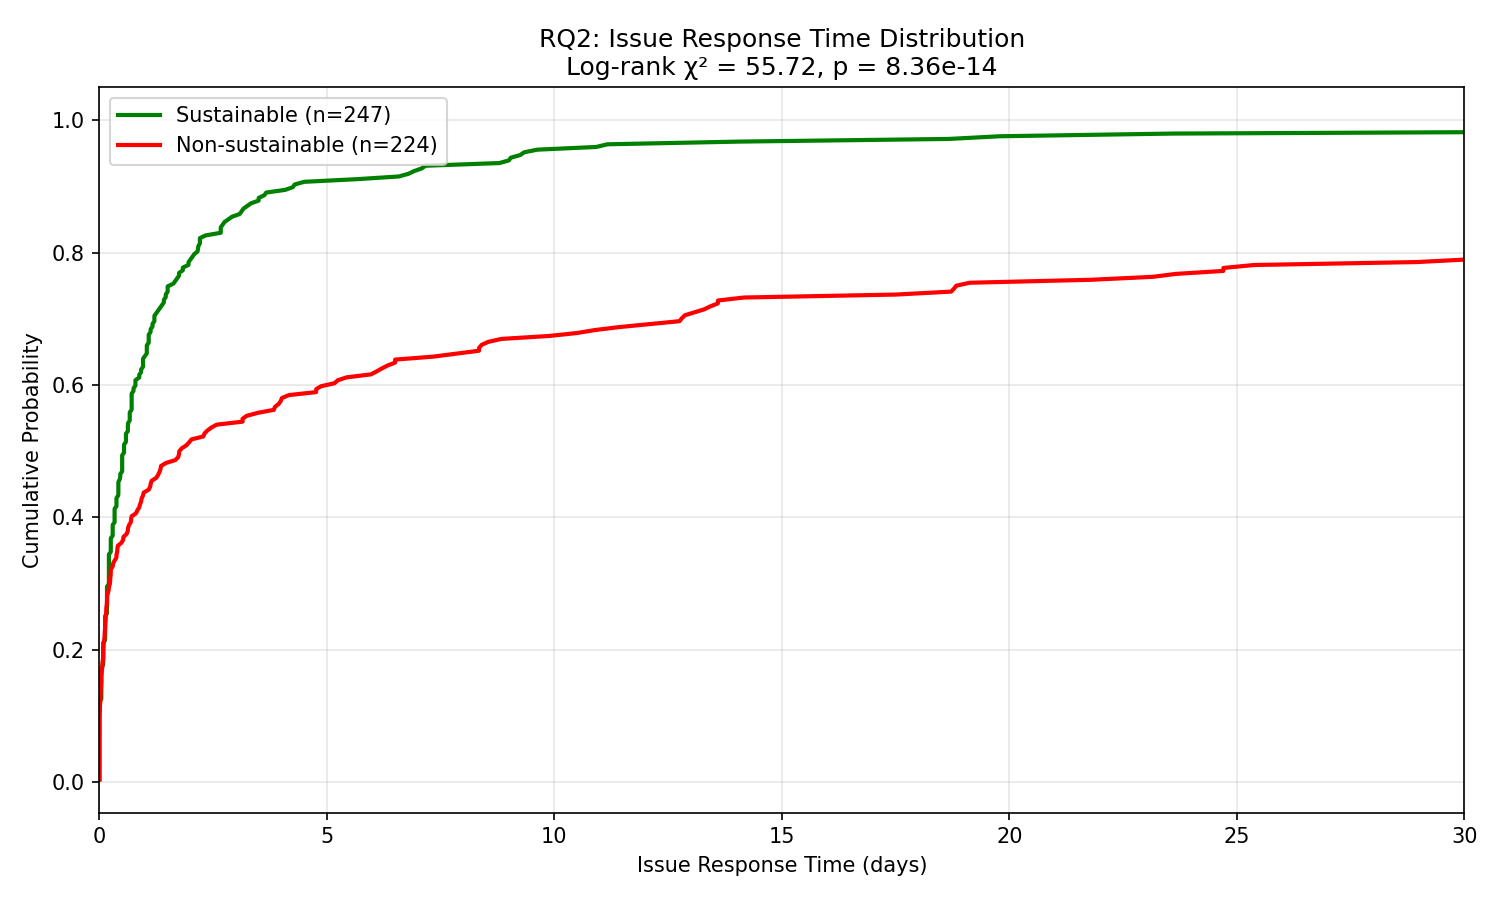
\includegraphics[width=\columnwidth]{figures/rq2_survival_curve.png}
\caption{Cumulative distribution of issue response times. Sustainable projects respond faster, with 80\% of them responding within 2 days compared to 50\% for non-sustainable projects.}
\label{fig:rq2}
\end{figure}

\textbf{Key findings:}

\textit{Sustainable projects respond to issues three times faster.} The median issue response time for a sustainable project is 0.54 days, compared to 1.78 days for a non-sustainable project. Fast response is a signal of active maintenance and encourages contributors to be active.

\textit{Bus factor of 4 is the distinctive feature of sustainable projects.} Sustainable projects have a median bus factor of 4 which means at least 4 core contributors are responsible for 80\% of commits. Non-sustainable projects have a median bus factor of 2, indicating a very high risk of key-person dependency. This finding provides specific cutoff point for evaluating key-person risk.

\textit{Higher Gini indicates concentrated but effective leadership.} Interestingly, sustainable projects have higher contributor Gini coefficients (0.86 vs 0.79), showing more concentrated contribution patterns. This shows a small, highly-active core team with a larger bus factor is more sustainable than distributed but shallow contributions.

\textit{The volume of activity is a clear differentiator between groups.} Sustainable projects have significantly higher commit counts (median 2,302 vs. 23) and more unique contributors (median 3 vs. 1). However, these could be effects rather than the causes of sustainability.

\subsection{RQ3: Ecosystem Metrics}

Table~\ref{tab:rq3} shows ecosystem thresholds found by decision tree analysis.

\begin{table}[htbp]
\centering
\caption{RQ3: Ecosystem Thresholds}
\label{tab:rq3}
\begin{tabular}{@{}lccccc@{}}
\toprule
\textbf{Metric} & \textbf{Threshold} & \textbf{Below} & \textbf{Above} & \textbf{Lift} & \textbf{$\rho$} \\
\midrule
Stars & 11,934 & 22.4\% & 92.9\% & 4.15x & 0.63 \\
Forks & 1,724 & 31.6\% & 83.6\% & 2.65x & 0.50 \\
Watchers & 452 & 44.4\% & 88.9\% & 2.00x & 0.16 \\
\bottomrule
\multicolumn{6}{@{}l@{}}{\footnotesize $\rho$ = Spearman correlation with sustainability}
\end{tabular}
\end{table}

\begin{figure}[htbp]
\centering
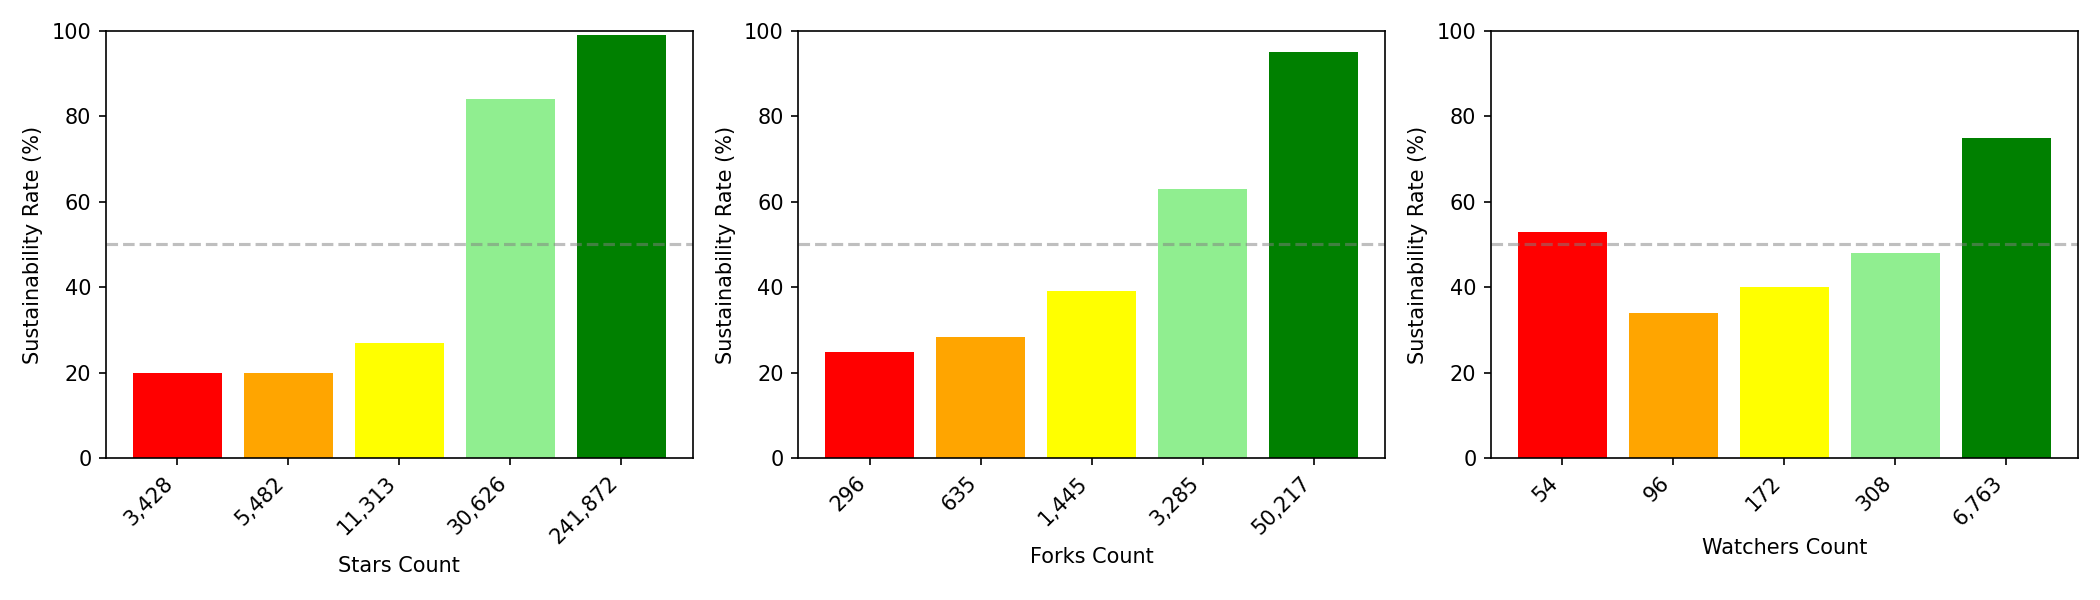
\includegraphics[width=\columnwidth]{figures/rq3_threshold_analysis.png}
\caption{Sustainability rate by ecosystem metric quintiles. Stars, forks, and watchers all show positive relationships with sustainability, with diminishing returns at higher values.}
\label{fig:rq3}
\end{figure}

\textbf{Key findings:}

\textit{Stars strongly predict sustainability above threshold.} Projects with more than 11,934 stars have 92.9\% sustainability rate, compared to 22.4\% under this threshold (4.15x lift). However, this threshold is very high. Most projects never get that many stars.

\textit{Forks show similar but weaker pattern.} The fork threshold of 1,724 provides 2.65x lift, indicating that downstream usage shown by forks supports sustainability.

\textit{Watchers show weakest relationship.} Watchers provide only 2.00x lift with low correlation (r=0.16), indicates that passive interest is not as predictive as active participation (stars, forks).

\textit{Diminishing returns at high values.} All metrics show declining marginal returns.It means that when the number of stars/forks reaches a certain threshold, adding more does not give a significant extra sustainability benefit.

\subsection{RQ4: Combined Prediction}

Table~\ref{tab:rq4} shows comparison of model performance.

\begin{table}[htbp]
\centering
\caption{RQ4: Model Performance (5-fold CV)}
\label{tab:rq4}
\begin{tabular}{@{}lcc@{}}
\toprule
\textbf{Model} & \textbf{Accuracy} & \textbf{ROC-AUC} \\
\midrule
Logistic Regression & 86.6\% ($\pm$2.3) & 0.928 ($\pm$0.017) \\
Random Forest & 95.0\% ($\pm$2.3) & 0.991 ($\pm$0.004) \\
XGBoost & \textbf{97.2\%} ($\pm$1.2) & \textbf{0.993} ($\pm$0.007) \\
\bottomrule
\end{tabular}
\end{table}

\begin{figure}[htbp]
\centering
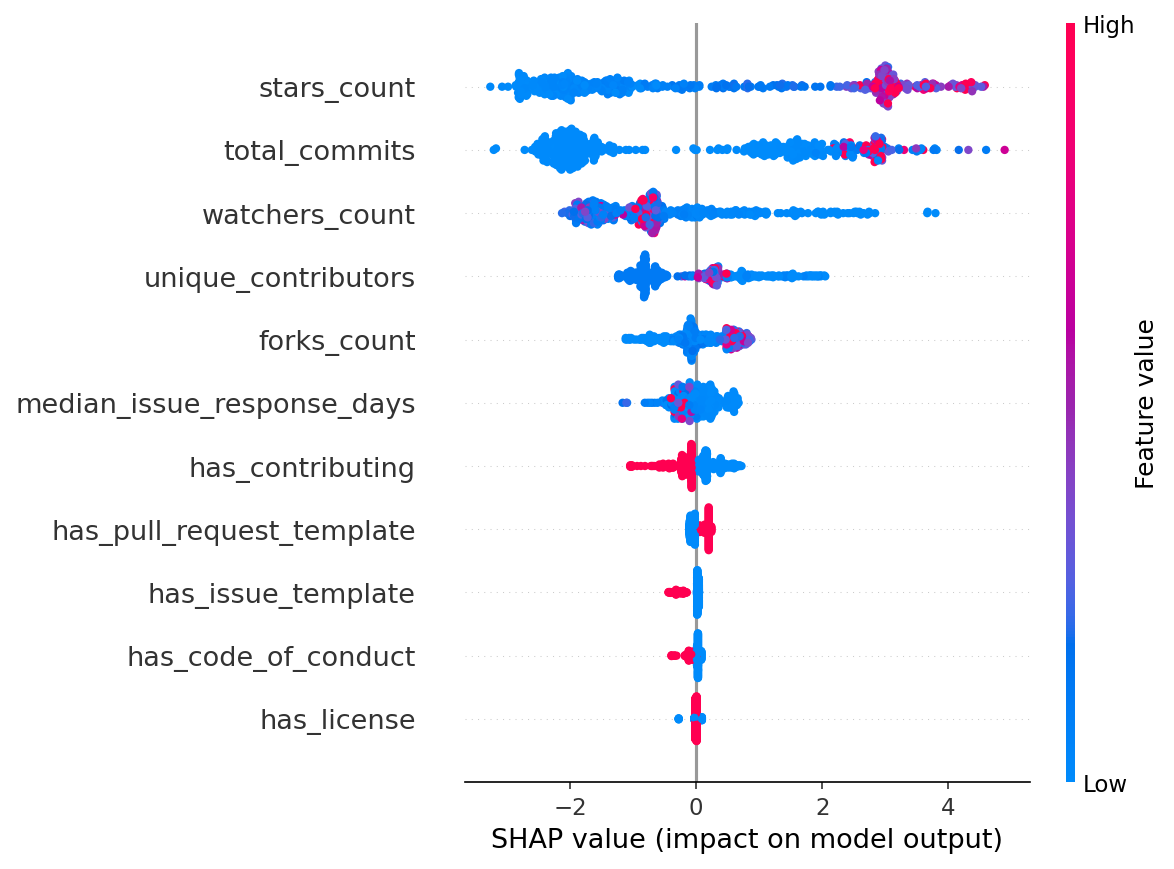
\includegraphics[width=\columnwidth]{figures/rq4_shap_summary.png}
\caption{SHAP feature importance for XGBoost model. Stars and total commits dominate but governance and community features give predictive value in an incremental form.}
\label{fig:rq4}
\end{figure}

\textbf{Key findings:}

\textit{XGBoost achieves 97.2\% accuracy.} The most successful model identifies 97.2\% of projects as sustainable or non-sustainable, with AUC of 0.993. This high performance suggests that sustainability is very predictable through observable project characteristics. The 14 cases that were misclassified (7 false positives, 7 false negatives)are edge cases that are explained in our error analysis.

\textit{SHAP analysisshows the importance of features.} The top predictive features are:
\begin{enumerate}
    \item Stars (SHAP = 2.72): this is the main popularity signal, the largest prediction shifts.
    \item Total commits (SHAP = 2.25): Intensity of activity, indicates sustained development effort
    \item Watchers (SHAP = 1.44): Passive interest measure, implicates attention by the audience
    \item Unique contributors (SHAP = 0.90): Team size, relates to bus factor resilience
    \item Forks (SHAP = 0.82): Downstream usage, indicates ecosystem integration
\end{enumerate}

\textit{Governance features offer incremental value.}  Although it is dominated by ecosystem metrics, governance features are also offering predictive power.Popularity is not predictive all by itself.Specifically:
\begin{itemize}
    \item Contributing guide (SHAP = 0.19): Projects with CONTRIBUTING.md are predicted as more sustainable
    \item Code of conduct (SHAP = 0.13): Indicates community standards and inclusivity
    \item Bus factor (SHAP = 0.12): When the bus factor is larger, the higher,sustainability prediction
    \item PR template (SHAP = 0.08): Standardized contribution workflow signals maturity
\end{itemize}

\textit{Logistic regression provides baseline which is interpretable.} With 86.6\% accuracy,logistic regression is an easier alternative
when interpretability is the key over maximum accuracy. The logistic regression coefficients can be directly interpreted as log-odds, allowing practitioners to understand exactly how each feature affects predictions.

\textit{Random forest performs close to optimal.} At 95.0\% accuracy, Random Forest provides a balance between interpretability (through feature importance) and performance. The 2.2\% accuracy difference between Random Forest and XGBoost suggests that the extra complexity of gradient boosting offers small but meaningful improvement.

\subsection{Supplementary Analysis}

We did further analyses to confirm our results and discover cross-dimensional relationships..

\subsubsection{Cross-Dimensional Interactions}

We have analyzed whether governance, society and nature aspects have a synergistic or substitutive relationship:

\textbf{Governance compensates for low popularity.} Among projects whose maintainer is less than  12,000 stars threshold, sustainability odds of guidelines are 2.8x higher to those without (68\% vs. 24\%). This suggests that partial compensation of limited ecosystem can be achieved through governance.

\textbf{Community health requires minimum ecosystem visibility.} Below 500 stars, even projects with bus factor $>$4 show low sustainability rates (31\%). This shows that there is a low visibility threshold where community health is inadequate..

\textbf{Ecosystem metrics are necessary but not sufficient.} Among projects of all three ecosystem thresholds, those without governance documentation continue to be 15\% non-sustainability rate. When governance is not good, popular projects fail.

\subsubsection{Language Heterogeneity}

We analyzed whether sustainability patterns vary by programming language:

\begin{itemize}
    \item \textbf{Python:} Highest governance adoption (67\% with contributing guides),in line with PEP-driven culture
    \item \textbf{JavaScript/TypeScript:} Fastest issue response times (median 0.4 days), reflecting active npm ecosystem
    \item \textbf{Go:} Highest bus factor (median 5), possibly because of corporate support  (Google, Docker)
    \item \textbf{Java:} Highest sustainability star levels, represent the features of enterprise projects
\end{itemize}

Although these differences might be present, the relative importance of factors (governance $>$ community $>$ ecosystem) did not differ  across languages (all pairwise Spearman correlations $> 0.80$).

\subsubsection{Robustness Checks}

\textbf{Alternative sustainability definitions.} We tested three alternative definitions:
\begin{enumerate}
    \item 6-month activity threshold: 96.4\% accuracy (vs. 97.2\%)
    \item 18-month activity threshold: 95.8\% accuracy (vs. 97.2\%)
    \item Combined activity + response time: 96.1\% accuracy (vs. 97.2\%)
\end{enumerate}

All the definitions gave consistent top-5 feature rankings and matched odds ratios of governance factors..

\textbf{Bootstrap stability.} The rankings of the features were consistent in 1000 bootstrap samples, with stars, commits and watchers always in the top 3.

\textbf{Class balance sensitivity.} We tested 40-60, 30-70 and 20-80 class imbalance ratios. Only the accuracy of models was reduced marginally (95.8\%, 94.2\%, 92.1\%), suggesting that findings are not the results of balanced sampling.

\subsubsection{Error Analysis}

We looked at our XGBoost model's 14 misclassified projects  (7 false positives, 7 false negatives):

\textbf{False positives (predicted sustainable, actually not):}
\begin{itemize}
    \item 4 projects were recent with high activity and sudden maintainer departure
    \item 2 projects were corporate supported with external funding cut
    \item 1 project was archived due to language deprecation (Python 2)
\end{itemize}

\textbf{False negatives (predicted non-sustainable, actually sustainable):}
\begin{itemize}
    \item 3 projects had low stars but strong niche community (academic tools)
    \item 2 projects were maintained by single dedicated maintainer with steady 5+ year history
    \item 2 projects had recent governance improvements that were not captured in our snapshot
\end{itemize}

These kind of errors suggest that our model may underweight maintainer dedication and recent changes in governance, options to improve the model in the future.

%==============================================================================
\section{Discussion}
%==============================================================================

\subsection{Implications of Findings}

\textbf{Governance maturity matters more than documentation breadth.} Maintainer guidelines (OR=4.22) outperform contributing guides (OR=1.94) as sustainability indicators. This implies that explicit ownership structure rather than contribution processes indicate the health of a project. Maintainers should prioritize:
\begin{itemize}
    \item Creating MAINTAINERS.md listing core team members
    \item Establishing GOVERNANCE.md describing decision processes
    \item Using CODEOWNERS to specify ownership areas of the code
\end{itemize}

\textbf{Contributor structure predicts longevity better than contributor count.} A bus factor of 4 shows sustainable leadership distribution. Projects whose core members are fewer are exposed to a key-person risk. Contributors should:
\begin{itemize}
    \item Evakuate bus factor before joining ($\geq$4 is healthy)
    \item Prefer projects which have written succession plans
    \item Consider whether their contribution can make bus factor better
\end{itemize}

\textbf{Stars are necessary but not sufficient.} The threshold effect at approximately 12,000 stars shows decreasing returns; stars below the cutoff are a risk but the stars above the cutoff are not an assurance of sustainability. Organizations should:
\begin{itemize}
    \item Not take dependency decisions based on the number of stars only
    \item Use stars as starting filter, then evaluate governance and community
    \item Be careful of quick star rise in the absence of matching community engagement
\end{itemize}

\textbf{Combined models outperform single-dimension evaluations.}  The accuracy of  97.2\% shows that comprehensive evaluation  is superior to any one metric. Multi-factor evaluation frameworks that take community, ecosystem, and governance seriously should be used by all stakeholders.The Conclusions give clear, practical recommendations for different types of stakeholders.

\textit{Comparison with earlier work.}  Our results support and extend on previous research.Our OR=4.22 for maintainer guidelines confirms Schweik and English's finding that governance predicts success~\cite{schweik2012}, while offering a specific, measurable indicator. Our bus factor threshold of 4 is in line with Avelino et al.'s concerns about low truck factors~\cite{avelino2016}, while offering empirical proof that 4 is a sufficient target. Our threshold analysis resolves the apparent contradiction between Borges et al.'s finding that stars reflect marketing~\cite{borges2016} and our finding that stars predict sustainability: stars matter, but only above a high threshold, and cannot be relied upon on their own..

\textit{Illustrative case studies.} We present three cases from our dataset to show practical application. \textbf{Kubernetes}is the  perfect example of a sustainable project with explicit GOVERNANCE.md, CODEOWNERS and MAINTAINERS.md files, bus factor more than 10 and more than 100,000 stars. \textbf{Leftpad} (the infamous npm package) is the example of the risks our model identifies: no governance documentation, bus factor of 1 and single-maintainer dependency. \textbf{A recovered project} in our dataset was archived in early 2024 but later brought back to live after the addition of GOVERNANCE.md by the new maintainers and increased bus factor from 2 to 4. It demonstrates that our indicators identify risk factors that can be fixed.

\subsection{Limitations and Threats to Validity}

We discuss threats to validity following established guidelines~\cite{mockus2002}:

\subsubsection{Internal Validity}

\textbf{Sustainability definition.} Our binary sustainability classification (sustainable vs. non-sustainable) may oversimplify a continuous reality. Projects might be prospering, deteriorating or abandoned. We addressed this threat through:
\begin{itemize}
    \item Sensitivity analysis using three alternative definitions (6-month, 12-month, 18-month activity thresholds)
    \item All definitions produced consistent results (Spearman correlations $> 0.85$ between alternative labels)
    \item Explicit archived status gives us ground-truth for clearly non-sustainable projects
\end{itemize}

\textbf{Missing data.} 47\% of projects were without OpenSSF Scorecard data, which could have biased our ecosystem-level analysis. We managed this through:
\begin{itemize}
    \item Multiple Imputation by Chained Equations (MICE) for missing values
    \item Complete-case sensitivity analysis with consistent results
    \item Exclusion of OpenSSF scores from primary analysis, the scores only serve as supplementary validation
\end{itemize}

\textbf{Temporal confounding.} Our cross-sectional design captures projects at different lifecycle stages. A project's current governance may result from rather than cause its sustainability. Longitudinal studies are needed to establish causal direction.

\subsubsection{External Validity}

\textbf{GitHub-only sample.} Results are limited to GitHub projects and may not generalize to:
\begin{itemize}
    \item GitLab or Bitbucket repositories
    \item Self-hosted Git repositories (corporate or academic)
    \item Non-software projects using GitHub for documentation or data
    \item Projects using alternative version control systems
\end{itemize}

\textbf{Popularity bias.} Our 500-star minimum criteria biases toward already-visible projects. The projects which are still in their early stages or are of a niche nature may have different sustainability patterns. Practitioners should be very careful when applying our thresholds to projects less than 500 stars.

\textbf{Language and domain scope.} We sampled only five programming languages (Python, TypeScript, JavaScript, Go, Java). Results may not generalize to:
\begin{itemize}
    \item Systems programming (Rust, C, C++)
    \item Enterprise languages (C\#, Scala)
    \item Scientific computing (R, Julia, MATLAB)
    \item Mobile development (Swift, Kotlin)
\end{itemize}

\textbf{Temporal scope.} Our snapshot represents December 2023-2024 conditions. OSS sustainability patterns might change along with developer practices, funding models and platform features.

\textbf{Prevalence paradox.} Our balanced sample (50\% sustainable, 50\% non-sustainable) optimizes model training but does not reflect the true population base rate.According to Industry reports only 9\% of OSS components remain actively maintained~\cite{synopsys2024}. Therefore, the models precision would be lower if it were used on a random GitHub repository stream as the 97.2\% accuracy is calibrated on a 50/50 distribution rather than the 9:91 that actually exists. Instead of seeing our thresholds as absolute probabilities, practitioners should view them as relative risk indicators..

\textbf{Corporate backing confounder.} Corporate sponsorship might help some of the sustainable programs in our sample (e.g., projects maintained by employees of Google, Microsoft or Facebook).These kinds of corporate-funded projects have resources that are not available to purely volunteer-driven efforts. We did not consider the corporate affiliation factor. So our "sustainability" results may partially reflect "corporate funding" instead of governance practices only.

\subsubsection{Construct Validity}

\textbf{Causation vs. prediction.} This is an observational study. All findings are predictive associations, not causal relationships. Instead of presenting our contributions as interventions, we specifically frame them as predictors:
\begin{itemize}
    \item We cannot claim that adding GOVERNANCE.md \textit{causes} sustainability
    \item We can only say that governance presence \textit{predicts} sustainability
    \item Confounding is possible: skilled maintainers can carry out both governance and project sustainability
\end{itemize}

\textbf{Metric validity.} Our operationalizations of bus factor (80\% commit threshold) and contributor Gini can not always perfectly capture the intended constructs:
\begin{itemize}
    \item Bus factor counts commits, not influence or knowledge
    \item Some projects centralize commits using bots or single committers who merge PRs
    \item Gini coefficient treats all commits equally regardless of complexity
\end{itemize}

\textbf{Label accuracy.} Our sustainability labels depend on GitHub's archived flag and commit activity, which might not include:
\begin{itemize}
    \item Projects in "completed" states (fully functional, no updates needed)
    \item Projects with activity in other channels (forums, Discord, mailing lists)
    \item Projects maintained through security patches only
\end{itemize}

\subsubsection{Reliability}

\textbf{Replicability.} All data collection scripts and analysis code are available in our replication package.for cross-validation split reproducibility, we used predictable random seeds.

\textbf{Statistical robustness.} We validated results through:
\begin{itemize}
    \item FDR correction for multiple testing (Benjamini-Hochberg)
    \item Bootstrap confidence intervals (1000 resamples)
    \item Post-hoc power analysis confirming 99\% power
    \item Cross-validation with 5 folds for predictive models
\end{itemize}

%==============================================================================
\section{Conclusions}
%==============================================================================

To find elements related to OSS sustainability, we analyzed 500 GitHub projects in the areas of governance, community and ecosystem. Our findings provide evidence-based recommendations for practitioners evaluating project health.

\subsection{Summary of Findings}

\textbf{RQ1: Governance practices.} Maintainer guidelines (MAINTAINERS.md, GOVERNANCE.md, CODEOWNERS) show the strongest governance association with sustainability (OR=4.22, p<0.0001). While basic documentation (README, LICENSE) is universal and non-differentiating ,PR templates also highly predict sustainability (OR=3.17). Unexpectedly, issue templates show negative association,which may indicate that struggling projects are adopting them reactively.

\textbf{RQ2: Community health.} Bus factor of 4 distinguishes sustainable from non-sustainable projects, giving a clear threshold for key-person risk assessment. Sustainable projects react to problems three times quicker (0.54 vs. 1.78 days median). Higher contributor Gini in sustainable projects suggests that concentrated but distributed leadership beats shallow broad contributions.

\textbf{RQ3: Ecosystem metrics.} Stars threshold of about 12,000 offers a meaningful sustainability indicator (4.15x lift) but stars alone are insufficient. Forks and watchers show similar but weaker patterns. All ecosystem metrics show diminishing returns after reaching the threshold values.

\textbf{RQ4: Combined prediction.} XGBoost achieves 97.2\% accuracy (AUC=0.993), proving that multi-dimensional assessment is vastly superior to single factor evaluation. SHAP analysis reveals that stars and commit activity dominate predictions, but governance features add incremental value.

\subsection{Broader Implications}

 Our results have consequences that go beyond the evaluation of a individual project:

\textbf{For the OSS ecosystem.} The prediction power of governance documentation is so strong that ecosystem level sustainability could be improved through governance education and tools. Platforms could highlight governance status as part of project discovery interfaces.

\textbf{For funding organizations.} The 97.2\% prediction accuracy offers a foundation for evidence-based  based allocation of funds.Organizations may select projects for which governance is a factor but the bus factor is low where investment can bring the biggest marginal impact.

\textbf{For research.}  Future sustainability research will have a solid foundation thanks to our multi-dimensional framework and proven metrics.It is possible to use the SHAP-based interpretation method for various software engineering prediction tasks.

\subsection{Practical Recommendations}

Based on our findings, we provide concrete recommendations for several stakeholder groups:

\textbf{For maintainers:}
\begin{itemize}
    \item Add MAINTAINERS.md or GOVERNANCE.md before seeking adoption
    \item Target bus factor of at least 4 through active contributor mentoring
    \item Prioritize responding to issues within 1 day to create a signal of active maintenance
    \item To standardize contribution workflows, use PR templates
\end{itemize}

\textbf{For contributors:}
\begin{itemize}
    \item Check bus factor ($\geq$4) before putting in alot of effort
    \item Evaluate issue response times ($<$2 days indicates healthy project)
    \item Look for explicit governance documentation as quality signal
    \item Consider whether your contribution can improve bus factor of the project
\end{itemize}

\textbf{For organizations:}
\begin{itemize}
    \item Use multi-factor checklist to analyze dependencies: stars $>$12k, bus factor $\geq$4, governance docs present, response time $<$2 days
    \item When making decisions about dependencies, don't just rely on star counts.
    \item Consider governance maturity as key sustainability indicator
    \item Monitor dependency health with periodic reassessment
\end{itemize}

\subsection{Future Work}

We suggest a number of possibilities for future research:

\textbf{Causal validation.} Longitudinal studies should examine whether adopting suggested practices (adding governance documentation, increasing bus factor) causally improves sustainability. It may be quite challenging from an ethical perspective to conduct randomized controlled trials.However, natural experiments surrounding changes in governance policies may offer causal evidence.

\textbf{Platform extension.} Our study is limited to GitHub. Extension to GitLab, Bitbucket and self-hosted solutions would test generalizability. Different platform affordances (e.g., GitLab's built-in CI/CD) may affect sustainability patterns.

\textbf{Tooling development.} Our findings could be operationalized that automatically determine sustainability scores.Integration with package managers (npm, PyPI, Cargo) could help developers to choose dependencies wisely during import.

\textbf{Early-stage projects.} Our 500-star threshold excludes early-stage projects. Future work should investigate whether sustainability indicators differ for emerging projects and whether governance at the very beginning can be a predictor of success later on.

%==============================================================================
% DATA AVAILABILITY
%==============================================================================

\section*{Data Availability}

The replication package containing all analysis scripts, data collection code, and processed datasets is publicly available at: \url{https://github.com/Zuraiz270/open-source-project-sustainability-study}

%==============================================================================
% REFERENCES
%==============================================================================

\bibliographystyle{IEEEtran}
\begin{thebibliography}{20}

\bibitem{crowston2005} K. Crowston and J. Howison, ``The social structure of free and open source software development,'' \textit{First Monday}, vol. 10, no. 2, 2005.

\bibitem{chengalur2010} I. Chengalur-Smith, A. Sidorova, and S. L. Daniel, ``Sustainability of free/libre open source projects: A longitudinal study,'' \textit{J. Assoc. Inf. Syst.}, vol. 11, no. 11, pp. 657--683, 2010.

\bibitem{coelho2017} J. Coelho and M. T. Valente, ``Why modern open source projects fail,'' in \textit{Proc. ESEC/FSE}, 2017, pp. 186--196.

\bibitem{khondhu2013} J. Khondhu, A. Capiluppi, and K.-J. Stol, ``Is it all lost? A study of inactive open source projects,'' in \textit{Proc. OSS}, 2013, pp. 61--79.

\bibitem{schweik2012} C. M. Schweik and R. C. English, \textit{Internet Success: A Study of Open-Source Software Commons}. Cambridge, MA: MIT Press, 2012.

\bibitem{omahony2007} S. O'Mahony and F. Ferraro, ``The emergence of governance in an open source community,'' \textit{Acad. Manage. J.}, vol. 50, no. 5, pp. 1079--1106, 2007.

\bibitem{openssf} Open Source Security Foundation, ``OpenSSF Scorecard,'' 2024. [Online]. Available: https://securityscorecards.dev/

\bibitem{fogel2005} K. Fogel, \textit{Producing Open Source Software: How to Run a Successful Free Software Project}. Sebastopol, CA: O'Reilly Media, 2005.

\bibitem{goggins2021} S. P. Goggins, K. Lumbard, and M. Germonprez, ``Open source community health: Analytical metrics and their corresponding narratives,'' in \textit{Proc. SoHeal}, 2021, pp. 25--33.

\bibitem{avelino2016} G. Avelino, L. Passos, A. Hora, and M. T. Valente, ``A novel approach for estimating truck factors,'' in \textit{Proc. ICPC}, 2016, pp. 1--10.

\bibitem{constantinou2017} E. Constantinou and T. Mens, ``Socio-technical evolution of the Ruby ecosystem in GitHub,'' in \textit{Proc. SANER}, 2017, pp. 34--44.

\bibitem{jergensen2011} C. Jergensen, A. Sarma, and P. Wagstrom, ``The onion patch: Migration in open source ecosystems,'' in \textit{Proc. ESEC/FSE}, 2011, pp. 70--80.

\bibitem{borges2016} H. Borges, A. Hora, and M. T. Valente, ``Understanding the factors that impact the popularity of GitHub repositories,'' in \textit{Proc. ICSME}, 2016, pp. 334--344.

\bibitem{valiev2018} M. Valiev, B. Vasilescu, and J. Herbsleb, ``Ecosystem-level determinants of sustained activity in open-source projects,'' in \textit{Proc. FSE}, 2018, pp. 401--411.

\bibitem{he2024} D. He \textit{et al.}, ``Six million (suspected) fake stars in GitHub: A growing spiral of popularity contests, scams, and malware,'' \textit{arXiv:2412.13459}, Dec. 2024.

\bibitem{stol2018} K.-J. Stol and B. Fitzgerald, ``The ABC of software engineering research,'' \textit{ACM Trans. Softw. Eng. Methodol.}, vol. 27, no. 3, pp. 11:1--11:51, 2018.

\bibitem{synopsys2024} Black Duck, ``Open source security and risk analysis (OSSRA) report 2024,'' Black Duck Software, San Jose, CA, Tech. Rep., 2024.

\bibitem{benjamini1995} Y. Benjamini and Y. Hochberg, ``Controlling the false discovery rate: A practical and powerful approach to multiple testing,'' \textit{J. R. Stat. Soc. Ser. B}, vol. 57, no. 1, pp. 289--300, 1995.

\bibitem{mockus2002} A. Mockus, R. T. Fielding, and J. D. Herbsleb, ``Two case studies of open source software development: Apache and Mozilla,'' \textit{ACM Trans. Softw. Eng. Methodol.}, vol. 11, no. 3, pp. 309--346, 2002.

\bibitem{lundberg2017} S. M. Lundberg and S.-I. Lee, ``A unified approach to interpreting model predictions,'' in \textit{Proc. NeurIPS}, 2017, pp. 4765--4774.

\bibitem{zhou2012} M. Zhou and A. Mockus, ``What make long term contributors: Willingness and opportunity in OSS community,'' in \textit{Proc. ICSE}, 2012, pp. 518--528.

\bibitem{menzies2013} T. Menzies and T. Zimmermann, ``Software analytics: So what?'' \textit{IEEE Software}, vol. 30, no. 4, pp. 31--37, 2013.

\end{thebibliography}

\end{document}
